\documentclass[a4paper,12pt]{article}

% polyglossia should go first!
\usepackage{polyglossia} % multi-language support
\setmainlanguage{russian}
\setotherlanguage{english}
\PolyglossiaSetup{english}{indentfirst=true}
\PolyglossiaSetup{russian}{indentfirst=true}

\defaultfontfeatures{Mapping=tex-text} % for converting "--" and "---"
\setmainfont{CMU Serif}
\setsansfont{CMU Sans Serif}
\setmonofont{CMU Typewriter Text}

\usepackage{minted}
\newcommand{\inputmintedbr}[2]{\inputminted[breaklines=true]{#1}{#2}}

% Опционно, требует  apt-get install scalable-cyrfonts.*
% и удаления одной строчки в cyrtimes.sty
% Сточку не удалять!
% \usepackage{cyrtimes}

% Картнки и tikz
\usepackage{graphicx}
\usepackage{tikz}
\usetikzlibrary{snakes,arrows,shapes}


% Некоторая русификация.
%\usepackage{misccorr}
\usepackage{indentfirst}
\renewcommand{\labelitemi}{\normalfont\bfseries{--}}

% Увы, поля придётся уменьшить из-за листингов.
\topmargin -1cm
\oddsidemargin -0.5cm
\evensidemargin -0.5cm
\textwidth 17cm
\textheight 24cm

\sloppy

% Оглавление в PDF
\usepackage[
bookmarks=true,
colorlinks=true, linkcolor=black, anchorcolor=black, citecolor=black, menucolor=black,filecolor=black, urlcolor=black,
unicode=true
]{hyperref}

% Для исходного кода в тексте
\newcommand{\Code}[1]{\textbf{#1}}

%\usepackage{verbatim}
%\usepackage{fancyvrb}
%\fvset{frame=leftline, fontsize=\small, framerule=0.4mm, rulecolor=\color{darkgray}, commandchars=\\\{\}}
%\renewcommand{\theFancyVerbLine}{\small\arabic{FancyVerbLine}}

%tables
\usepackage{tabu}
\usepackage{multirow}

\title{Отчёт по лабораторной работе \\ <<IP-маршрутизация>>}
\author{Гребенюк Александр Андреевич}

\begin{document}

\maketitle

\tableofcontents

\clearpage

% Текст отчёта должен быть читаемым!!! Написанное здесь является рыбой.

\section{Топология сети}

Топология сети и использыемые IP-адреса показаны на рис.~\ref{fig:network}.

\begin{figure}[h]
\centering
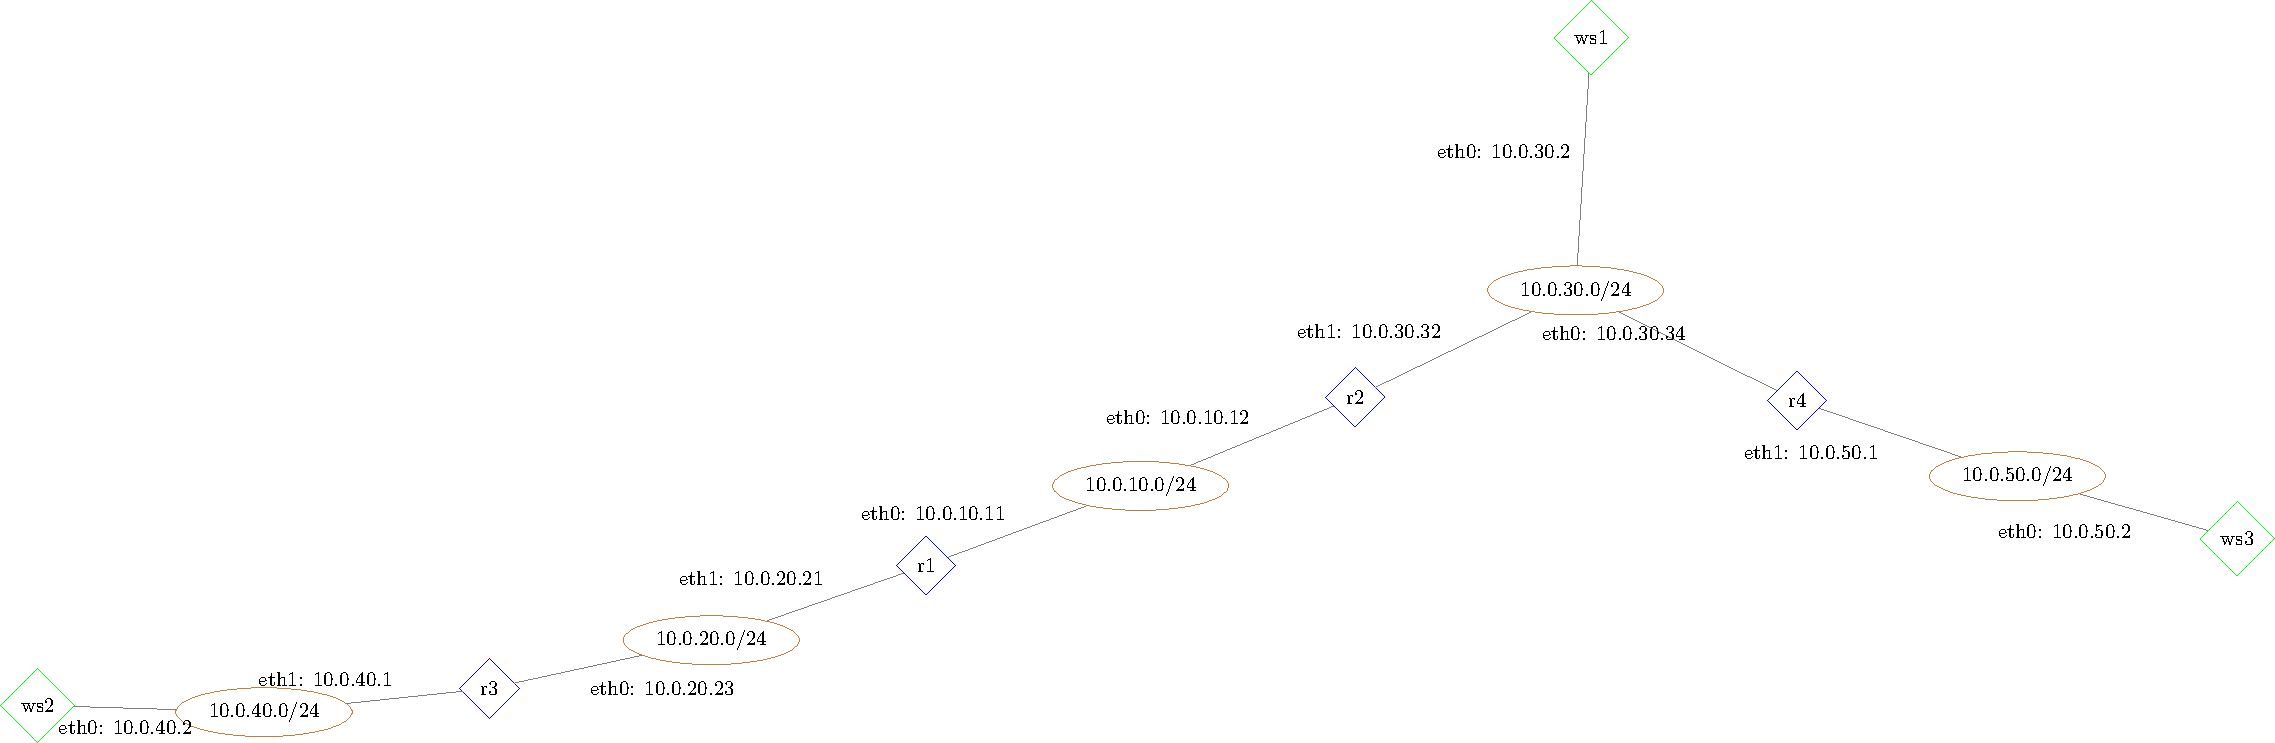
\includegraphics[width=\textwidth]{includes/network_gv.pdf}
\caption{Топология сети}
\label{fig:network}
\end{figure}


\section{Назначение IP-адресов}
\begin{itemize}
\item Ниже приведён файл настройки протокола IP маршрутизатора \textbf{r1}.
\lstinputlisting{../../net/r1/etc/network/interfaces}
\item Ниже приведён файл настройки протокола IP маршрутизатора \textbf{r2}.
\lstinputlisting{../../net/r2/etc/network/interfaces}
\item Ниже приведён файл настройки протокола IP маршрутизатора \textbf{r3}.
\lstinputlisting{../../net/r3/etc/network/interfaces}
\item Ниже приведён файл настройки протокола IP маршрутизатора \textbf{r4}.
\lstinputlisting{../../net/r4/etc/network/interfaces}

\item Ниже приведён файл настройки протокола IP рабочей станции \textbf{ws1}.
\lstinputlisting{../../net/ws1/etc/network/interfaces}
\item Ниже приведён файл настройки протокола IP рабочей станции \textbf{ws2}.
\lstinputlisting{../../net/ws2/etc/network/interfaces}
\item Ниже приведён файл настройки протокола IP рабочей станции \textbf{ws3}.
\lstinputlisting{../../net/ws3/etc/network/interfaces}
\end{itemize}


\section{Таблица маршрутизации}
\begin{itemize}
\item Таблица маршрутизации \textbf{r1}.
\lstinputlisting{../../results/r1.route}

\item Таблица маршрутизации \textbf{r2}.
\lstinputlisting{../../results/r2.route}

\item Таблица маршрутизации \textbf{r3}.
\lstinputlisting{../../results/r3.route}

\item Таблица маршрутизации \textbf{r4}.
\lstinputlisting{../../results/r4.route}
\end{itemize}


\section{Проверка настройки сети}
\begin{itemize}
\item Вывод \textbf{traceroute} от узла \textbf{ws1} до \textbf{ws2} при нормальной работе сети.
\lstinputlisting{../../results/ws12.trace}
\item Вывод \textbf{traceroute} от узла \textbf{ws1} до \textbf{ws3} при нормальной работе сети.
\lstinputlisting{../../results/ws13.trace}
\item Вывод \textbf{traceroute} от узла \textbf{ws2} до \textbf{ws3} при нормальной работе сети.
\lstinputlisting{../../results/ws23.trace}
\end{itemize}


\section{Маршрутизация}

\begin{table}[h]
\caption{MAC-адреса}
  \begin{tabu} to \textwidth {|X|X|X|}
  \hline
  Host & Interface & MAC  \\
  \hline
  ws1 & eth0 & 7e:a6:65:cd:a1:ab \\
  \hline
  ws2 & eth0 & 42:70:9a:0b:39:80 \\
  \hline
  \multirow{2}{*}{r1} & eth0 & be:14:9b:41:0f:21 \\
                      & eth1 & 3a:bf:72:36:29:d9 \\
  \hline
  \multirow{2}{*}{r2} & eth0 & ca:a0:5b:a0:0e:20 \\
                      & eth1 & 96:e8:1f:21:5e:44 \\
  \hline
  \multirow{2}{*}{r3} & eth0 & ee:93:78:86:e8:49 \\
                      & eth1 & 76:e5:80:0f:a1:02 \\
  \hline
  \end{tabu}
\end{table}

% На пути здесь достаточно быть одному аршрутизатору!

\begin{itemize}
\item Таблица маршрутизации \textbf{r1}.
\lstinputlisting{../../results/r1.route}

\item Таблица маршрутизации \textbf{r2}.
\lstinputlisting{../../results/r2.route}

\item Таблица маршрутизации \textbf{r3}.
\lstinputlisting{../../results/r3.route}
\end{itemize}

Показаны опыты после стирания кеша ARP.
% Не забудьте это сделать!


\textbf{ws1} выполняет команду
\begin{lstlisting}
ping 10.0.40.2 -c 1
\end{lstlisting}

По таблице маршрутизации вычисляется, что \textbf{ws1} не имеет возможности непосредственно отправить ICMP-запрос в подсеть 10.0.40.0/24. Поэтому ICMP-запрос отпраляется на маршрутизатор, IP-адрес которого известен из таблицы маршрутизации, но неизвестен MAC-адрес. Для определения MAC-адреса отправляется широковещательный ARP-запрос в интерфейс eth0, на который приходит ответ от \textbf{r2}.
\lstinputlisting{../../results/indirect_routing/ws1.eth0.log}

Аналогичным образом \textbf{r2} широковещательным ARP-запросом опрашивает интерфейс eth1(исходя из таблицы маршрутищации) и получает ответ от \textbf{r1} c его MAC-адресом, что позволяет направить ICMP-запрос (c TTL-1) далее.
\lstinputlisting{../../results/indirect_routing/r2.eth1.log}

Аналогичным образом \textbf{r1} отправляет ICMP-запрос на \textbf{r3}.
\lstinputlisting{../../results/indirect_routing/r2.eth0.log}
\lstinputlisting{../../results/indirect_routing/r1.eth0.log}

Аналогичным образом \textbf{r3} отпрявляет ICMP-запрос на \textbf{ws2}
\lstinputlisting{../../results/indirect_routing/r1.eth1.log}
\lstinputlisting{../../results/indirect_routing/r3.eth0.log}

\textbf{ws2} получает ICMP-запрос и отправляет ICMP-ответ. На обратном пути следования ответа нет необходимости направлять широковещательные ARP-запросы для поиска MAC-адресов, т.к. ARP-кеш является заполненным.
\lstinputlisting{../../results/indirect_routing/ws2.eth0.log}

\section{Продолжительность жизни пакета}
Добавим кольцо между \textbf{r1} и \textbf{r2}:
\lstinputlisting{../../results/ttl_test/break_r1.sh}

Получим таблицу маршрутизации \textbf{r1}:
\lstinputlisting{../../results/ttl_test/r1.route}

Отправим ICMP-запрос c \textbf{ws1} на \textbf{ws2}:
\lstinputlisting{../../results/ttl_test/ws1.cmd.log}

Воспользуемся командой tcpdump:
\textbf{ws1}:
\lstinputlisting{../../results/ttl_test/ws1.eth0.log}
\textbf{r2.eth1}:
\lstinputlisting{../../results/ttl_test/r2.eth1.log}
\textbf{r2.eth0}:
\lstinputlisting{../../results/ttl_test/r2.eth0.log}
\textbf{r1}:
\lstinputlisting{../../results/ttl_test/r1.eth0.log}

\textbf{r1} отправил сообщение о превышении времени жизни.

\section{Изучение IP-фрагментации}
\textbf{ws1}
\begin{lstlisting}
ip l set mtu 500 dev eth0
\end{lstlisting}

\textbf{r2}
\begin{lstlisting}
ip l set mtu 500 dev eth1
\end{lstlisting}
% Напоминаем, что PMTU следует отключить!

\textbf{r1}
\begin{lstlisting}
ping 10.0.30.2 -c 1 -s 1000
\end{lstlisting}

Вывод \textbf{tcpdump} на маршрутизаторе \textbf{r2} перед сетью с уменьшенным MTU.
\lstinputlisting{../../results/mtu_test/r2.eth1.log}

Вывод \textbf{tcpdump} на маршрутизаторе \textbf{r2} после сети с уменьшенным MTU.
\lstinputlisting{../../results/mtu_test/r2.eth0.log}

Вывод \textbf{tcpdump} на узле получателя \textbf{ws1}.
\lstinputlisting{../../results/mtu_test/ws1.eth0.log}


\section{Отсутствие сети}
\lstinputlisting{../../results/network_ureachable}


\section{Отсутствие IP-адреса в сети}
\lstinputlisting{../../results/destination_unreachable}

\end{document}
